\documentclass{article}
\usepackage{amsmath}
\usepackage{float}
\usepackage{amssymb}
\usepackage{graphicx}
\usepackage[margin=1in]{geometry}
\usepackage{multicol,listings}
\usepackage[font=small]{caption}
\usepackage{cite}
\usepackage{epstopdf}
\usepackage{caption}
\usepackage{subcaption}
\usepackage{float}
\usepackage{listings}
\usepackage{hyperref}
\bibliographystyle{plain}
\begin{document}
\input{titlepage.tex}
\newpage
\tableofcontents
\newpage
\section{Problem description}

%\begin{figure}[H]
%	\centering
%	\includegraphics[width=\textwidth]{toroid.eps}
%	\caption{Three-dimensional shape of our object of interest including relevant parameters depicting the radii describing the torus. In our case: $R=4,\rho=2$}
%	\label{toroid}
%\end{figure}

%\section{Introduction}

%\section{Trial wavefunction}
%\section{Working algorithm (Metropolis-Haestings)}
%\section{Reducing parameters}
%\section{Results}
Our goal is to find an upper bound for the energy of the ground state of the hydrogen molecule. To do this, we use the variational approach, which states that 
\begin{align}
E = \frac{{\left\langle \psi_{tr}  \right|\hat H\left| \psi_{tr}  \right\rangle }}{{\left\langle \psi_{tr}  \right|\left. \psi_{tr}  \right\rangle }} = \frac{{\int {d{{\vec r}_1}\int {d{{\vec r}_2}} {\psi_{tr} ^ * }\hat H\psi_{tr} } }}{{\left\langle \psi_{tr}  \right|\left. \psi_{tr}  \right\rangle }} \ge {E_g}.
\label{eq:main}
\end{align}
Our goal is now to evaluate this integral with the help of the Monte Carlo method. 
\subsection{Variational (Quantum) Monte Carlo}
Monte Carlo integration is based on the random sampling of the integrands evaluation points. For higher dimensional integrals this method converges faster than standard numerical methods as the distribution uniformity of the random points is higher than for example a cubical grid. To improve on this integration scheme the integral should be rewritten in a form where we can sample over a distribution close to the shape of the integrand, this ensures that the regions that contribute strongly to the integral are evaluated more exactly. This method is called importance sampling Monte Carlo and will be used in our evaluation of the hydrogen molecule’s energy. \\
In our case we would like to sample over  $|{\phi _{tr}}{|^2}$ as it will be close to the integrand in the energy expression $\phi _{_{tr}}^*H{\phi _{tr}}$. To achieve this the Metropolis-Hastings algorithm will be used.\\
\subsubsection{Metropolis-Hastings}
To sample from the probability distribution (${p \propto |{\psi _{tr}}{|^2}}$) needed to calculate the integral we use the Metropolis-Hastings algorithm, which is a Markov chain Monte Carlo based method~\cite{robert2013monte}. The main advantage of this method is that we do not have to normalize the wavefunction as this algorithm draws from a valid (normalized) probability distribution proportional to the function supplied (in our case ${|{\psi _{tr}}{|^2}}$). The general algorithm as implemented in our code can be stated as:
\begin{enumerate}
\item randomly initiate the values for ${\overrightarrow {{r_1}} }$ and ${\overrightarrow {{r_2}} }$ 
\item  propose new ${\overrightarrow {{r_1}} }$ and ${\overrightarrow {{r_2}} }$ by stepping both vectors in a random direction where the step size is drawn from a normal distribution
\item calculate the acceptance ratio: $|{\psi _{tr}}|_{new}^2/|{\psi _{tr}}{|^2}$
\item if the ratio is bigger than one accept the new coordinates, if the ratio is smaller than one accept with probability given by the ratio
\end{enumerate}
For the convergence of this algorithm we will have to make smart decisions for the step size used in  step two. It is important to not have the step size too small as then the coordinate space will be traced out slowly. The same thing will happen if the step size is too big because then the acceptance rate will be low. In our code the standard deviation for the step size is updated according to
\begin{align}
\sigma  = \sigma  + \delta  (A - 0.5),
\end{align}
A is the average acceptance rate and $\delta$ is a factor between zero and one, in our case we have used $\delta=0.05$. This will push the acceptance rate towards 50\% ensuring fast convergence of the algorithm.



\subsection{Hamiltonian of the hydrogen molecule}
Before we use this method, however, we have to rewrite Equation~\ref{eq:main} somewhat. We start by writing down the Hamiltonian for the hydrogen molecule. We assume that the protons do not move (Born-Oppenheimer approximation). Then the Hamiltonian consists of two single-electron Hamiltonians and two extra terms to account for electron-electron repulsion and proton-proton repulsion respectively. This gives the following result:
\begin{align}	   
\hat H =& {\hat H_1} + {\hat H_2} + {\hat H_{ee}} + {\hat H_{pp}}\\
\hat H =& \left( { - \frac{{{\hbar ^2}}}{{2m}}\nabla _1^2 - \frac{{{e^2}}}{{4\pi {\varepsilon _0}}}\frac{1}{{{r_{1L}}}} - \frac{{{e^2}}}{{4\pi {\varepsilon _0}}}\frac{1}{{{r_{1R}}}}} \right) + \left( { - \frac{{{\hbar ^2}}}{{2m}}\nabla _2^2 - \frac{{{e^2}}}{{4\pi {\varepsilon _0}}}\frac{1}{{{r_{2L}}}} - \frac{{{e^2}}}{{4\pi {\varepsilon _0}}}\frac{1}{{{r_{2R}}}}} \right)\nonumber\\
& + \left( {\frac{{{e^2}}}{{4\pi {\varepsilon _0}}}\frac{1}{{{r_{12}}}}} \right) + \left( {\frac{{{e^2}}}{{4\pi {\varepsilon _0}}}\frac{1}{{{r_{LR}}}}} \right).
\end{align}\\
In this equation we have defined ${r_{1L}} = \left| {{{\vec r}_1} - {{\vec r}_L}} \right|$, etc., where $r_L$ is the position vector of the left-most proton. To simplify the units somewhat, we introduce atomic units, where lengths are given in terms of the Bohr radius and energies are given in terms of twice the ionization energy of hydrogen:
\begin{align}
{a_0} =& \frac{{4\pi {\varepsilon _0}{\hbar ^2}}}{{m{e^2}}} = 0.529\mathring{A}\\
E =& 2 \cdot \frac{{{e^2}}}{{4\pi {\varepsilon _0}{a_0}}} = 2 \cdot \left( { - 13.6eV} \right) =  - 27.2eV
\end{align}\\
In these units, we can write the Hamiltonian as follows \cite{MSU_paper}:
\begin{align}
\hat H =  - \frac{1}{2}\left( {\nabla _1^2 + \nabla _2^2} \right) - \frac{1}{{{r_{1L}}}} - \frac{1}{{{r_{1R}}}} - \frac{1}{{{r_{2L}}}} - \frac{1}{{{r_{2R}}}} + \frac{1}{{{r_{12}}}} + \frac{1}{{{r_{LR}}}}
\end{align}
Now, we can choose our axes in such a way that the two protons are located symmetrically along the x-axis at $-s/2$ and $+s/2$, with $s$ the separation between the protons. In that case, we can write the distances between an electron and a proton as
\begin{align}
{r_{1L}} =& \left| {{{\vec r}_1} + \frac{s}{2}\hat x} \right|\\{r_{1R}} =& \left| {{{\vec r}_1} - \frac{s}{2}\hat x} \right|
\end{align}
Now that we have the Hamiltonian, we can now try to write down a trial wave function to use for variational calculus. Luckily, this has already been done, so we can immediately write down the final result\cite{MSU_paper}:
\begin{align}
\Psi \left( {{{\vec r}_1},{{\vec r}_2}} \right) = {\phi _1}\left( {{{\vec r}_1}} \right){\phi _2}\left( {{{\vec r}_2}} \right)\psi_{tr} \left( {{{\vec r}_1},{{\vec r}_2}} \right)
\end{align}
The trial wave function consists of two single-electron terms (one that only depends on $r_1$, and one that only depends on $r_2$) and an interaction term $\psi_{tr}$. The single-electron wave functions are given by
\begin{align}
{\phi _1}\left( {{{\vec r}_1}} \right) =& {e^{ - {{{r_{1L}}} \mathord{\left/
 {\vphantom {{{r_{1L}}} a}} \right.
 \kern-\nulldelimiterspace} a}}} + {e^{ - {{{r_{1R}}} \mathord{\left/
 {\vphantom {{{r_{1R}}} a}} \right.
 \kern-\nulldelimiterspace} a}}} = {\phi _{1L}} + {\phi _{1R}},\\
 {\phi _2}\left( {{{\vec r}_2}} \right) =& {e^{ - {{{r_{2L}}} \mathord{\left/
 {\vphantom {{{r_{2L}}} a}} \right.
 \kern-\nulldelimiterspace} a}}} + {e^{ - {{{r_{2R}}} \mathord{\left/
 {\vphantom {{{r_{2R}}} a}} \right.
 \kern-\nulldelimiterspace} a}}} = {\phi _{2L}} + {\phi _{2R}}.
\end{align}
These wave functions correspond to two non-interacting electrons orbiting two protons. However, this does not accurately describe our system. We must also add an interaction term
\begin{align}
\psi_{tr} \left( {{{\vec r}_1},{{\vec r}_2}} \right) = {e^{\frac{{\left| {{{\vec r}_1} - {{\vec r}_2}} \right|}}{{\alpha \left( {1 + \beta \left| {{{\vec r}_1} - {{\vec r}_2}} \right|} \right)}}}}
\end{align}
In this term, $\alpha$ and $\beta$ are parameters that we will optimize to find the minimum of the energy through the variational approach.\\
\newpage
\subsection{Local energy}
Now we re-examine the integral that we want to evaluate (Equation \ref{eq:main}) in the variational approach, which is
\begin{align}
E = \frac{{\int {d{{\vec r}_1}\int {d{{\vec r}_2}} {\psi_{tr} ^ * }\hat H\psi_{tr} } }}{{\left\langle \psi_{tr}  \right|\left. \psi_{tr}  \right\rangle }} = \int {d{{\vec r}_1}\int {d{{\vec r}_2}} \frac{{{\psi_{tr} ^ * }\psi_{tr} }}{{\left\langle \psi_{tr}  \right|\left. \psi_{tr}  \right\rangle }} \cdot \frac{{\hat H\psi_{tr} }}{\psi_{tr} }}
\label{eq:var_int}.
\end{align}
We define the local energy $\epsilon$ and the weight $\omega$ as
\begin{align}
\varepsilon \left( {{{\vec r}_1},{{\vec r}_2},s} \right) =& \frac{{\hat H\psi_{tr} }}{\psi_{tr} },\\
\omega \left( {{{\vec r}_1},{{\vec r}_2},s} \right) =& \frac{{{{\left| \psi_{tr}  \right|}^2}}}{{\left\langle \psi_{tr}  \right|\left. \psi_{tr}  \right\rangle }}.
\end{align}
Then we can write the integral of Equation \ref{eq:var_int} as 
\begin{align}
E = \int {d{{\vec r}_1}\int {d{{\vec r}_2}} \omega \left( {{{\vec r}_1},{{\vec r}_2},s} \right)\varepsilon \left( {{{\vec r}_1},{{\vec r}_2},s} \right)}.
\end{align}
Our final step is to write down the local energy of the system. The derivation of the local energy is a bit of work (see \cite{MSU_paper} or appendix A), but eventually one can find as final result
\begin{align}
\varepsilon  =&  - \frac{1}{{{a^2}}} + \frac{1}{{a{\phi _1}}}\left[ {\frac{{{\phi _{1L}}}}{{{r_{1L}}}} + \frac{{{\phi _{1R}}}}{{{r_{1R}}}}} \right] + \frac{1}{{a{\phi _2}}}\left[ {\frac{{{\phi _{2L}}}}{{{r_{2L}}}} + \frac{{{\phi _{2R}}}}{{{r_{2R}}}}} \right] + \left( {\frac{{{\phi _{1L}}{{\hat r}_{1L}} + {\phi _{1R}}{{\hat r}_{1R}}}}{{{\phi _1}}} - \frac{{{\phi _{2L}}{{\hat r}_{2L}} + {\phi _{2R}}{{\hat r}_{2R}}}}{{{\phi _2}}}} \right)\left( {\frac{{{{\hat r}_{12}}}}{{2a{\gamma ^2}}}} \right)\nonumber\\
 &- \frac{{\left( {1 + 4\beta } \right){r_{12}} + 4}}{{4{\gamma ^4}{r_{12}}}} - \frac{1}{{{r_{1L}}}} - \frac{1}{{{r_{1R}}}} - \frac{1}{{{r_{2L}}}} - \frac{1}{{{r_{2R}}}} + \frac{1}{{{r_{12}}}} + \frac{1}{{{r_{LR}}}}.
\end{align}
Now, it is important to note that this result is not always bounded. Since we do not want a solution that blows up, we can derive a set of conditions to keep the solution bounded. While deriving the local energy, we have already found one condition for the case $r_{12}\rightarrow0$, namely $\alpha=0$.
We also have a condition for the case $r_{1L}\rightarrow0$:
\begin{align}
\mathop {\lim }\limits_{{r_{1L}} \to 0} \left| \varepsilon  \right| < \infty  &\Rightarrow \frac{1}{{a{\phi _1}}}\left[ {\frac{{{\phi _{1L}}}}{{{r_{1L}}}}} \right] - \frac{1}{{{r_{1L}}}} = 0\nonumber\\& \Rightarrow \frac{{{e^{ - {r_{1L}}/a}}}}{{a\left( {{e^{ - {r_{1L}}/a}} + {e^{ - {r_{1R}}/a}}} \right)}} = 1\nonumber\\&
 \Rightarrow a = \frac{1}{{1 + {e^{ - \left| {{{\vec r}_L} - {{\vec r}_R}} \right|/a}}}}.
\end{align}
The other possibilities ($r_{1R}\rightarrow0$, etc) give the same condition, which is called the Coulomb cusp condition. With this condition, we can now eliminate $a$ as a variable from the local energy by solving the above equation.
However, this is easier said than done. The non-linear form of this equation means that it is not possible to solve for a analytically. Therefore, we use Newton-Rhapson to numerically find the value for a for which the above equation holds.
\noindent The iteration scheme for Newton-Rhapson is given by
\begin{align}
{a^{n + 1}} = {a^n} - \frac{{f\left( {{a^n}} \right)}}{{f'\left( {{a^n}} \right)}},
\end{align}
where $f$ is given by
\begin{align}
f'\left( a \right) = \frac{1}{{1 + {e^{ - s/a}}}} - a.
\end{align}
We also need the derivative of f, which is
\begin{align}
f'\left( a \right) =  - \frac{{s{e^{ - s/a}}}}{{{{\left( {a + a{e^{ - s/a}}} \right)}^2}}} - 1.
\end{align}
Now we can use the above scheme to find the value of $a$ for a given $s$. Therefore, since we want to know the minimum of the local energy for every $s$, we only need to find one parameter, namely $\beta$. This parameter will now be found using the Monte Carlo method. 
\\
\newpage
\subsection{Steepest descent scheme}
After setting s the only free wave function parameter left is $\beta$, as explained above. To minimize the energy for beta a damped steepest descent scheme is used. In this scheme $\beta$ is updated according to
\begin{align}
\beta  &= \beta  - \gamma \frac{{d\left\langle E \right\rangle }}{{d\beta }},\\
\frac{{d\left\langle E \right\rangle }}{{d\beta }} &= 2\left[ {\left\langle {{E_L}\frac{{d\ln ({\psi _{tr}})}}{{d\beta }}} \right\rangle  + \left\langle {{E_L}} \right\rangle \left\langle {\frac{{d\ln ({\psi _{tr}})}}{{d\beta }}} \right\rangle } \right],
\end{align}
where we have used $\gamma=0.1$. For our trial wave function only the interaction term depends on $\beta$ so we have
\begin{align}
\frac{{d\ln ({\psi _{tr}})}}{{d\beta }} =  - \frac{{r_{12}^2}}{{2(1 + \beta {r_{12}})}}.
\end{align}
Now $\beta$ and also the acceptance rate can be updated after every M iterations until the local energy converges to its minimum.	

\section{Results}
After performing the simulations we can now gather the results. The simulations are done in two steps. First, 2,500,000 iterations are used to find equilibrium, where both $\beta$ and the step size are continuously updated as explained above. After equilibrium has been reached, 10,000,000 iterations are used to calculate the energy. This process is repeated for 50 values of the separation s between 1 and 2 a.u. This gives the following result:
\begin{figure}[H]
	\centering
	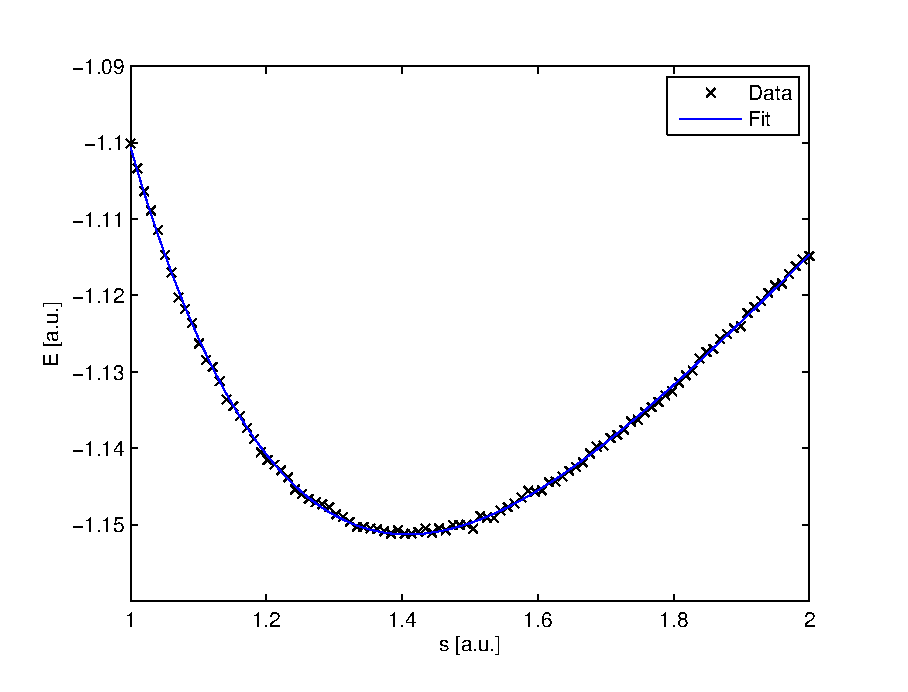
\includegraphics[width=0.8\textwidth]{plot.eps}
	\caption{The total energy of the hydrogen molecule calculated using Variational Monte Carlo (black crosses). The blue fitted line is the Morse potential, given in Equation~\ref{eq:Morse}.}
	\label{plot}
\end{figure}
\newpage
\noindent  In this plot, the data points calculated by the simulation are shown. We have also fitted these data points with a so-called Morse potential. This potential is given by
\begin{align}
V = D{\left( {1 - {e^{ - a\left( {s - {s_0}} \right)}}} \right)^2} - {V_0}.
\label{eq:Morse}
\end{align}
In this expression, $D$ is the dissociation energy, $s_0$ is the equilibrium separation, $V_0$ is the equilibrium energy and $a$ is given by
\begin{align}
a = \sqrt{\frac{K}{2D}},
\end{align}
with K the spring constant of the potential. At this point, it is good to note that there are two ways to find the dissociation energy D. One can find it directly through the fit parameters, or one can use:
\begin{align}
D = {V_0} - 1.
\end{align}
In this report, we use the expression above to find D. The reason for this is that both the parameters $a$ and $D$ have a similar effect on the form of the potential. Therefore, when only examining a small part of the total potential, these parameters can be rather uncertain. $V_0$, on the other hand, fits the lowest part of the curve (the part we are most interested in) much better, as it does not care for the rest of the curve. Therefore, we use $V_0$ to find a value for the dissociation energy.\\
The spectrum of the Morse potential can be calculated analytically. This gives~\cite{jose_pdf}:
\begin{align}
{E_n} = \hbar \omega \left( {n + \frac{1}{2}} \right)\left( {1 - \frac{{\hbar \omega \left( {n + \frac{1}{2}} \right)}}{{4D}}} \right),
\end{align}
with $\omega=\sqrt{\frac{K}{M}}$, where M is the reduced mass of the hydrogen molecule. In atomic units, we can write\newline M = 925.260 a.u.\cite{hyplink}. By fitting the data points we have found, we can now find values for these parameters and compare the results:
\begin{table}[H]
\centering
\begin{tabular}{|l|l|}
\hline
\textit{Parameter} & \textit{Result {[}a.u.{]}} \\ \hline
\textbf{Results}   &                            \\\hline
$D$                  & 0.1512 $\pm$ 0.0001              \\\hline
$R_0$                 & 1.408  $\pm$0.002              \\\hline
$\hbar\omega$               & 0.02037 $\pm$0.00007                            \\\hline
\textbf{Results simulation Jose}                   &                            \\\hline
$D$                   &       0.15123(3)                     \\\hline
$R_0$                   &           1.4054(2)                 \\\hline
 $\hbar\omega$                  &      0.02044(2)                      \\\hline
 \textbf{Literature}                  &                            \\\hline
  $D$                 &   0.1645(6)                         \\\hline
    $R_0$               &      1.40111(9)                      \\\hline
     $\hbar\omega$               &     0.02005(3)          \\          
     \hline
\end{tabular}
\caption{Values for the parameters $D$, $R_0$ and $\hbar\omega$ found with fitting our data points, from the simulation performed by Jose~\cite{jose_pdf} and literature ($D$ taken from~\cite{traynor1991}, $R_0$ and $\hbar\omega$ from~\cite{jose_pdf}).}
\end{table}
\newpage
\subsection{Discussion}
Comparing our results with the results of a similar simulation by Jose and with the literature, we see that our results are quite comparable to the results obtained by Jose, but we also see that the literature values are somewhat different. 

The fact that our results are very similar to those found by Jose makes a lot of sense, as our approach is almost exactly the same. The good agreement does indicate that our simulation is working as intended, however, so it is still useful to do this comparison. One difference between the two approaches is the number of walkers used. We used fewer walkers than Jose, meaning that we needed more iterations to find the results. 

The agreement of our results with values found in literature is less good, however. The separation distance and oscillation frequency are quite reasonable, but the dissociation energy is rather low. The most probable explanation for this is that there are extra effects that we have not taken into account. This would mean that our trial wave function is not as good as we think it is, leading to a less tight lower bound for the dissociation energy. It is good to note that the fact that our value of the dissociation energy is lower at least indicates that our approach is valid, as we are looking for a lower bound for the dissociation energy (since the total energy is negative, an upper bound for the energy corresponds to a lower bound for the dissociation energy).

A couple of things could be done in order to improve our simulation. First of all, more iterations could be used to calculate the energy. More iterations could be used per point to reduce the uncertainty per point, and more values of the separation distance could be used to increase the accuracy of the fit. Alternatively, more walkers could be used. This has a very similar effect to using more iterations, and would improve the result in a similar way.

More drastically, one could try to find a better trial wave function for the hydrogen molecule. As discussed above, the upper bound found for the energy is not particularly impressive for variational calculus. Therefore, finding a better trial wave function may yield a tighter upper bound, improving the results of the simulation. However, finding a good trial wave function can be rather difficult, making this a rather drastic option. 






\newpage
%We know that the self energy is given by:
\begin{align}
\varepsilon  =  &- \frac{1}{{{a^2}}} + \frac{1}{{a{\phi _1}}}\left[ {\frac{{{\phi _{1L}}}}{{{r_{1L}}}} + \frac{{{\phi _{1R}}}}{{{r_{1R}}}}} \right] + \frac{1}{{a{\phi _2}}}\left[ {\frac{{{\phi _{2L}}}}{{{r_{2L}}}} + \frac{{{\phi _{2R}}}}{{{r_{2R}}}}} \right] + \left( {\frac{{{\phi _{1L}}{{\hat r}_{1L}} + {\phi _{1R}}{{\hat r}_{1R}}}}{{{\phi _1}}} - \frac{{{\phi _{2L}}{{\hat r}_{2L}} + {\phi _{2R}}{{\hat r}_{2R}}}}{{{\phi _2}}}} \right)\left( {\frac{{{{\hat r}_{12}}}}{{2a{\gamma ^2}}}} \right)\nonumber\\&
 - \frac{{\left( {1 + 4\beta } \right){r_{12}} + 4}}{{4{\gamma ^4}{r_{12}}}} - \frac{1}{{{r_{1L}}}} - \frac{1}{{{r_{1R}}}} - \frac{1}{{{r_{2L}}}} - \frac{1}{{{r_{2R}}}} + \frac{1}{{{r_{12}}}} + \frac{1}{{{r_{LR}}}}
\end{align}
Since we do not want this expression to explode, we must have certain conditions on the variational parameters. For example:
\begin{align}{l}
\mathop {\lim }\limits_{{r_{1L}} \to 0} \left| \varepsilon  \right| < \infty  &\Rightarrow \frac{1}{{a{\phi _1}}}\left[ {\frac{{{\phi _{1L}}}}{{{r_{1L}}}}} \right] - \frac{1}{{{r_{1L}}}} = 0\nonumber\\& \Rightarrow \frac{{{e^{ - {r_{1L}}/a}}}}{{a\left( {{e^{ - {r_{1L}}/a}} + {e^{ - {r_{1R}}/a}}} \right)}} = 1\nonumber\\&
 \Rightarrow a = \frac{1}{{1 + {e^{ - \left| {{{\vec r}_L} - {{\vec r}_R}} \right|/a}}}}
\end{align}
For $r_{1R}$, etc. we find the same condition. With this condition, we can now eliminate $a$ as a variable from the self energy by solving the above equation.\\
However, this is easier said than done. The non-linear form of this equation means that it is not possible to solve for a analytically. Therefore, we use Newton-Rhapson to numerically find the value for a for which the above equation holds. The iteration scheme for Newton-Rhapson is given by
\begin{align}
{a^{n + 1}} = {a^n} - \frac{{f\left( {{a^n}} \right)}}{{f\left( {{a^n}} \right)}},
\end{align}
where $f$ is given by
\begin{align}
f\left( a \right) = \frac{1}{{1 + {e^{ - \left| {{{\vec r}_L} - {{\vec r}_R}} \right|/a}}}} - a.
\end{align}
We also need the derivative of f
\begin{align}
f'\left( a \right) =  - \frac{{\left| {{{\vec r}_L} - {{\vec r}_R}} \right|{e^{ - \left| {{{\vec r}_L} - {{\vec r}_R}} \right|/a}}}}{{{{\left( {a + a{e^{ - \left| {{{\vec r}_L} - {{\vec r}_R}} \right|/a}}} \right)}^2}}} - 1.
\end{align}












\newpage
%
\newpage
%To sample from the probability distribution (${p \propto |{\psi _{tr}}{|^2}}$) needed to calculate the integral we use the Metropolis-Hastings algorithm, which is a Markov chain Monte Carlo based method~\cite{robert2013monte}. The main advantage of this method is that we do not have to normalize the wavefunction as this algorithm draws from a valid (normalized) probability distribution proportional to the function supplied (in our case ${|{\psi _{tr}}{|^2}}$). The general algorithm as implemented in our code can be stated as:
\begin{enumerate}
\item randomly initiate the values for ${\overrightarrow {{r_1}} }$ and ${\overrightarrow {{r_2}} }$ 
\item  propose new ${\overrightarrow {{r_1}} }$ and ${\overrightarrow {{r_2}} }$ by stepping both vectors in a random direction where the step size is drawn from a normal distribution
\item calculate the acceptance ratio: $|{\psi _{tr}}|_{new}^2/|{\psi _{tr}}{|^2}$
\item if the ratio is bigger than one accept the new coordinates, if the ratio is smaller than one accept with probability given by the ratio
\end{enumerate}
For the convergence of this algorithm we will have to make smart decisions for the step size used in  step two. It is important to not have the step size too small as then the coordinate space will be traced out slowly. The same thing will happen if the step size is too big because then the acceptance rate will be low. In our code the standard deviation for the step size is updated according to
\begin{align}
\sigma  = \sigma  + \delta  (A - 0.5),
\end{align}
A is the average acceptance rate and $\delta$ is a factor between zero and one, in our case we have used $\delta=0.05$. This will push the acceptance rate towards 50\% ensuring fast convergence of the algorithm.



\newpage
%Our goal is to find an upper bound for the energy of the ground state of the hydrogen molecule. To do this, we use the variational approach, which states that 
\begin{align}
E = \frac{{\left\langle \psi_{tr}  \right|\hat H\left| \psi_{tr}  \right\rangle }}{{\left\langle \psi_{tr}  \right|\left. \psi_{tr}  \right\rangle }} = \frac{{\int {d{{\vec r}_1}\int {d{{\vec r}_2}} {\psi_{tr} ^ * }\hat H\psi_{tr} } }}{{\left\langle \psi_{tr}  \right|\left. \psi_{tr}  \right\rangle }} \ge {E_g}.
\label{eq:main}
\end{align}
Our goal is now to evaluate this integral with the help of the Monte Carlo method. 
\subsection{Variational (Quantum) Monte Carlo}
Monte Carlo integration is based on the random sampling of the integrands evaluation points. For higher dimensional integrals this method converges faster than standard numerical methods as the distribution uniformity of the random points is higher than for example a cubical grid. To improve on this integration scheme the integral should be rewritten in a form where we can sample over a distribution close to the shape of the integrand, this ensures that the regions that contribute strongly to the integral are evaluated more exactly. This method is called importance sampling Monte Carlo and will be used in our evaluation of the hydrogen molecule’s energy. \\
In our case we would like to sample over  $|{\phi _{tr}}{|^2}$ as it will be close to the integrand in the energy expression $\phi _{_{tr}}^*H{\phi _{tr}}$. To achieve this the Metropolis-Hastings algorithm will be used.\\
\subsubsection{Metropolis-Hastings}
To sample from the probability distribution (${p \propto |{\psi _{tr}}{|^2}}$) needed to calculate the integral we use the Metropolis-Hastings algorithm, which is a Markov chain Monte Carlo based method~\cite{robert2013monte}. The main advantage of this method is that we do not have to normalize the wavefunction as this algorithm draws from a valid (normalized) probability distribution proportional to the function supplied (in our case ${|{\psi _{tr}}{|^2}}$). The general algorithm as implemented in our code can be stated as:
\begin{enumerate}
\item randomly initiate the values for ${\overrightarrow {{r_1}} }$ and ${\overrightarrow {{r_2}} }$ 
\item  propose new ${\overrightarrow {{r_1}} }$ and ${\overrightarrow {{r_2}} }$ by stepping both vectors in a random direction where the step size is drawn from a normal distribution
\item calculate the acceptance ratio: $|{\psi _{tr}}|_{new}^2/|{\psi _{tr}}{|^2}$
\item if the ratio is bigger than one accept the new coordinates, if the ratio is smaller than one accept with probability given by the ratio
\end{enumerate}
For the convergence of this algorithm we will have to make smart decisions for the step size used in  step two. It is important to not have the step size too small as then the coordinate space will be traced out slowly. The same thing will happen if the step size is too big because then the acceptance rate will be low. In our code the standard deviation for the step size is updated according to
\begin{align}
\sigma  = \sigma  + \delta  (A - 0.5),
\end{align}
A is the average acceptance rate and $\delta$ is a factor between zero and one, in our case we have used $\delta=0.05$. This will push the acceptance rate towards 50\% ensuring fast convergence of the algorithm.



\subsection{Hamiltonian of the hydrogen molecule}
Before we use this method, however, we have to rewrite Equation~\ref{eq:main} somewhat. We start by writing down the Hamiltonian for the hydrogen molecule. We assume that the protons do not move (Born-Oppenheimer approximation). Then the Hamiltonian consists of two single-electron Hamiltonians and two extra terms to account for electron-electron repulsion and proton-proton repulsion respectively. This gives the following result:
\begin{align}	   
\hat H =& {\hat H_1} + {\hat H_2} + {\hat H_{ee}} + {\hat H_{pp}}\\
\hat H =& \left( { - \frac{{{\hbar ^2}}}{{2m}}\nabla _1^2 - \frac{{{e^2}}}{{4\pi {\varepsilon _0}}}\frac{1}{{{r_{1L}}}} - \frac{{{e^2}}}{{4\pi {\varepsilon _0}}}\frac{1}{{{r_{1R}}}}} \right) + \left( { - \frac{{{\hbar ^2}}}{{2m}}\nabla _2^2 - \frac{{{e^2}}}{{4\pi {\varepsilon _0}}}\frac{1}{{{r_{2L}}}} - \frac{{{e^2}}}{{4\pi {\varepsilon _0}}}\frac{1}{{{r_{2R}}}}} \right)\nonumber\\
& + \left( {\frac{{{e^2}}}{{4\pi {\varepsilon _0}}}\frac{1}{{{r_{12}}}}} \right) + \left( {\frac{{{e^2}}}{{4\pi {\varepsilon _0}}}\frac{1}{{{r_{LR}}}}} \right).
\end{align}\\
In this equation we have defined ${r_{1L}} = \left| {{{\vec r}_1} - {{\vec r}_L}} \right|$, etc., where $r_L$ is the position vector of the left-most proton. To simplify the units somewhat, we introduce atomic units, where lengths are given in terms of the Bohr radius and energies are given in terms of twice the ionization energy of hydrogen:
\begin{align}
{a_0} =& \frac{{4\pi {\varepsilon _0}{\hbar ^2}}}{{m{e^2}}} = 0.529\mathring{A}\\
E =& 2 \cdot \frac{{{e^2}}}{{4\pi {\varepsilon _0}{a_0}}} = 2 \cdot \left( { - 13.6eV} \right) =  - 27.2eV
\end{align}\\
In these units, we can write the Hamiltonian as follows \cite{MSU_paper}:
\begin{align}
\hat H =  - \frac{1}{2}\left( {\nabla _1^2 + \nabla _2^2} \right) - \frac{1}{{{r_{1L}}}} - \frac{1}{{{r_{1R}}}} - \frac{1}{{{r_{2L}}}} - \frac{1}{{{r_{2R}}}} + \frac{1}{{{r_{12}}}} + \frac{1}{{{r_{LR}}}}
\end{align}
Now, we can choose our axes in such a way that the two protons are located symmetrically along the x-axis at $-s/2$ and $+s/2$, with $s$ the separation between the protons. In that case, we can write the distances between an electron and a proton as
\begin{align}
{r_{1L}} =& \left| {{{\vec r}_1} + \frac{s}{2}\hat x} \right|\\{r_{1R}} =& \left| {{{\vec r}_1} - \frac{s}{2}\hat x} \right|
\end{align}
Now that we have the Hamiltonian, we can now try to write down a trial wave function to use for variational calculus. Luckily, this has already been done, so we can immediately write down the final result\cite{MSU_paper}:
\begin{align}
\Psi \left( {{{\vec r}_1},{{\vec r}_2}} \right) = {\phi _1}\left( {{{\vec r}_1}} \right){\phi _2}\left( {{{\vec r}_2}} \right)\psi_{tr} \left( {{{\vec r}_1},{{\vec r}_2}} \right)
\end{align}
The trial wave function consists of two single-electron terms (one that only depends on $r_1$, and one that only depends on $r_2$) and an interaction term $\psi_{tr}$. The single-electron wave functions are given by
\begin{align}
{\phi _1}\left( {{{\vec r}_1}} \right) =& {e^{ - {{{r_{1L}}} \mathord{\left/
 {\vphantom {{{r_{1L}}} a}} \right.
 \kern-\nulldelimiterspace} a}}} + {e^{ - {{{r_{1R}}} \mathord{\left/
 {\vphantom {{{r_{1R}}} a}} \right.
 \kern-\nulldelimiterspace} a}}} = {\phi _{1L}} + {\phi _{1R}},\\
 {\phi _2}\left( {{{\vec r}_2}} \right) =& {e^{ - {{{r_{2L}}} \mathord{\left/
 {\vphantom {{{r_{2L}}} a}} \right.
 \kern-\nulldelimiterspace} a}}} + {e^{ - {{{r_{2R}}} \mathord{\left/
 {\vphantom {{{r_{2R}}} a}} \right.
 \kern-\nulldelimiterspace} a}}} = {\phi _{2L}} + {\phi _{2R}}.
\end{align}
These wave functions correspond to two non-interacting electrons orbiting two protons. However, this does not accurately describe our system. We must also add an interaction term
\begin{align}
\psi_{tr} \left( {{{\vec r}_1},{{\vec r}_2}} \right) = {e^{\frac{{\left| {{{\vec r}_1} - {{\vec r}_2}} \right|}}{{\alpha \left( {1 + \beta \left| {{{\vec r}_1} - {{\vec r}_2}} \right|} \right)}}}}
\end{align}
In this term, $\alpha$ and $\beta$ are parameters that we will optimize to find the minimum of the energy through the variational approach.\\
\newpage
\subsection{Local energy}
Now we re-examine the integral that we want to evaluate (Equation \ref{eq:main}) in the variational approach, which is
\begin{align}
E = \frac{{\int {d{{\vec r}_1}\int {d{{\vec r}_2}} {\psi_{tr} ^ * }\hat H\psi_{tr} } }}{{\left\langle \psi_{tr}  \right|\left. \psi_{tr}  \right\rangle }} = \int {d{{\vec r}_1}\int {d{{\vec r}_2}} \frac{{{\psi_{tr} ^ * }\psi_{tr} }}{{\left\langle \psi_{tr}  \right|\left. \psi_{tr}  \right\rangle }} \cdot \frac{{\hat H\psi_{tr} }}{\psi_{tr} }}
\label{eq:var_int}.
\end{align}
We define the local energy $\epsilon$ and the weight $\omega$ as
\begin{align}
\varepsilon \left( {{{\vec r}_1},{{\vec r}_2},s} \right) =& \frac{{\hat H\psi_{tr} }}{\psi_{tr} },\\
\omega \left( {{{\vec r}_1},{{\vec r}_2},s} \right) =& \frac{{{{\left| \psi_{tr}  \right|}^2}}}{{\left\langle \psi_{tr}  \right|\left. \psi_{tr}  \right\rangle }}.
\end{align}
Then we can write the integral of Equation \ref{eq:var_int} as 
\begin{align}
E = \int {d{{\vec r}_1}\int {d{{\vec r}_2}} \omega \left( {{{\vec r}_1},{{\vec r}_2},s} \right)\varepsilon \left( {{{\vec r}_1},{{\vec r}_2},s} \right)}.
\end{align}
Our final step is to write down the local energy of the system. The derivation of the local energy is a bit of work (see \cite{MSU_paper} or appendix A), but eventually one can find as final result
\begin{align}
\varepsilon  =&  - \frac{1}{{{a^2}}} + \frac{1}{{a{\phi _1}}}\left[ {\frac{{{\phi _{1L}}}}{{{r_{1L}}}} + \frac{{{\phi _{1R}}}}{{{r_{1R}}}}} \right] + \frac{1}{{a{\phi _2}}}\left[ {\frac{{{\phi _{2L}}}}{{{r_{2L}}}} + \frac{{{\phi _{2R}}}}{{{r_{2R}}}}} \right] + \left( {\frac{{{\phi _{1L}}{{\hat r}_{1L}} + {\phi _{1R}}{{\hat r}_{1R}}}}{{{\phi _1}}} - \frac{{{\phi _{2L}}{{\hat r}_{2L}} + {\phi _{2R}}{{\hat r}_{2R}}}}{{{\phi _2}}}} \right)\left( {\frac{{{{\hat r}_{12}}}}{{2a{\gamma ^2}}}} \right)\nonumber\\
 &- \frac{{\left( {1 + 4\beta } \right){r_{12}} + 4}}{{4{\gamma ^4}{r_{12}}}} - \frac{1}{{{r_{1L}}}} - \frac{1}{{{r_{1R}}}} - \frac{1}{{{r_{2L}}}} - \frac{1}{{{r_{2R}}}} + \frac{1}{{{r_{12}}}} + \frac{1}{{{r_{LR}}}}.
\end{align}
Now, it is important to note that this result is not always bounded. Since we do not want a solution that blows up, we can derive a set of conditions to keep the solution bounded. While deriving the local energy, we have already found one condition for the case $r_{12}\rightarrow0$, namely $\alpha=0$.
We also have a condition for the case $r_{1L}\rightarrow0$:
\begin{align}
\mathop {\lim }\limits_{{r_{1L}} \to 0} \left| \varepsilon  \right| < \infty  &\Rightarrow \frac{1}{{a{\phi _1}}}\left[ {\frac{{{\phi _{1L}}}}{{{r_{1L}}}}} \right] - \frac{1}{{{r_{1L}}}} = 0\nonumber\\& \Rightarrow \frac{{{e^{ - {r_{1L}}/a}}}}{{a\left( {{e^{ - {r_{1L}}/a}} + {e^{ - {r_{1R}}/a}}} \right)}} = 1\nonumber\\&
 \Rightarrow a = \frac{1}{{1 + {e^{ - \left| {{{\vec r}_L} - {{\vec r}_R}} \right|/a}}}}.
\end{align}
The other possibilities ($r_{1R}\rightarrow0$, etc) give the same condition, which is called the Coulomb cusp condition. With this condition, we can now eliminate $a$ as a variable from the local energy by solving the above equation.
However, this is easier said than done. The non-linear form of this equation means that it is not possible to solve for a analytically. Therefore, we use Newton-Rhapson to numerically find the value for a for which the above equation holds.
\noindent The iteration scheme for Newton-Rhapson is given by
\begin{align}
{a^{n + 1}} = {a^n} - \frac{{f\left( {{a^n}} \right)}}{{f'\left( {{a^n}} \right)}},
\end{align}
where $f$ is given by
\begin{align}
f'\left( a \right) = \frac{1}{{1 + {e^{ - s/a}}}} - a.
\end{align}
We also need the derivative of f, which is
\begin{align}
f'\left( a \right) =  - \frac{{s{e^{ - s/a}}}}{{{{\left( {a + a{e^{ - s/a}}} \right)}^2}}} - 1.
\end{align}
Now we can use the above scheme to find the value of $a$ for a given $s$. Therefore, since we want to know the minimum of the local energy for every $s$, we only need to find one parameter, namely $\beta$. This parameter will now be found using the Monte Carlo method. 
\\

%Monte Carlo integration is based on the random sampling of the integrands evaluation points. For higher dimensional integrals this method converges faster than standard numerical methods as the distribution uniformity of the random points is higher than for example a cubical grid. To improve on this integration scheme the integral should be rewritten in a form where we can sample over a distribution close to the shape of the integrand, this ensures that the regions that contribute strongly to the integral are evaluated more exactly. This method is called importance sampling Monte Carlo and will be used in our evaluation of the hydrogen molecule’s energy. \\
In our case we would like to sample over  $|{\phi _{tr}}{|^2}$ as it will be close to the integrand in the energy expression $\phi _{_{tr}}^*H{\phi _{tr}}$. To achieve this the Metropolis-Hastings algorithm will be used.
\bibliography{bib}
\newpage
\section*{Appendix A}
\appendix
\noindent Our goal is to derive the local energy for the hydrogen molecule. We start with the trial wave function
\begin{align}
\Psi \left( {{{\vec r}_1},{{\vec r}_2}} \right) = {\phi _1}\left( {{{\vec r}_1}} \right){\phi _2}\left( {{{\vec r}_2}} \right)\psi \left( {{{\vec r}_1},{{\vec r}_2}} \right).
\end{align}\\
The trial wave function consists of two single-electron terms (one that only depends on $r_1$, and one that only depends on $r_2$) and an interaction term $\psi$. The single-electron wave functions are given by
\begin{align}
{\phi _1}\left( {{{\vec r}_1}} \right) = {e^{ - {{{r_{1L}}} \mathord{\left/
 {\vphantom {{{r_{1L}}} a}} \right.
 \kern-\nulldelimiterspace} a}}} + {e^{ - {{{r_{1R}}} \mathord{\left/
 {\vphantom {{{r_{1R}}} a}} \right.
 \kern-\nulldelimiterspace} a}}} = {\phi _{1L}} + {\phi _{1R}}\,\,\,\,,\,\,\,\,\,{\phi _2}\left( {{{\vec r}_2}} \right) = {e^{ - {{{r_{2L}}} \mathord{\left/
 {\vphantom {{{r_{2L}}} a}} \right.
 \kern-\nulldelimiterspace} a}}} + {e^{ - {{{r_{2R}}} \mathord{\left/
 {\vphantom {{{r_{2R}}} a}} \right.
 \kern-\nulldelimiterspace} a}}} = {\phi _{2L}} + {\phi _{2R}},
 \end{align}\\
 where we have defined
 \begin{align}
{r_{1L}} = \left| {{{\vec r}_1} - {{\vec r}_L}} \right|\,\,\,\,,\,\,\,etc
 \end{align}\\
 with $r_L$ the position vector for the left proton, etc. These wave functions correspond to non-interacting electrons orbiting two protons. However, this does not accurately describe our system. We must also add an interaction term:
 \begin{align}
 \psi \left( {{{\vec r}_1},{{\vec r}_2}} \right) = {e^{\frac{{\left| {{{\vec r}_1} - {{\vec r}_2}} \right|}}{{\alpha \left( {1 + \beta \left| {{{\vec r}_1} - {{\vec r}_2}} \right|} \right)}}}}
 \end{align}\\
 In this term, $\alpha$ and $\beta$ are parameters that we will optimize to find the minimum of the energy through the variational approach.\\

 Now, in order to calculate the energy of the system, we need to write down the Hamiltonian. In this case, the Hamiltonian consists of the Hamiltonian for two single electrons, with two extra terms for electron-electron interaction and proton-proton interaction:
  \begin{align}
  \hat H =& {{\hat H}_1} + {{\hat H}_2} + {{\hat H}_{ee}} + {{\hat H}_{pp}}\\
  \hat H =& \left( { - \frac{1}{2}\nabla _1^2 - \frac{1}{{{r_{1L}}}} - \frac{1}{{{r_{1R}}}}} \right) + \left( { - \frac{1}{2}\nabla _2^2 - \frac{1}{{{r_{2L}}}} - \frac{1}{{{r_{2R}}}}} \right) + \left( {\frac{1}{{{r_{12}}}}} \right) + \left( {\frac{1}{{{r_{LR}}}}} \right)
  \end{align}\\
 Introducing some notation gives:
 \begin{align}
 V =&  - \frac{1}{{{r_{1L}}}} - \frac{1}{{{r_{1R}}}} - \frac{1}{{{r_{2L}}}} - \frac{1}{{{r_{2R}}}} + \frac{1}{{{r_{12}}}} + \frac{1}{{{r_{LR}}}}\\
 \hat H =&  - \frac{1}{2}\nabla _1^2 - \frac{1}{2}\nabla _2^2 + V
 \end{align}\\
 Now we can use this Hamiltonian to find the local energy we are interested in. To this end, we apply the definition of the local energy:
 \begin{align}
 \varepsilon  = \frac{{\hat H\Psi \left( {{{\vec r}_1},{{\vec r}_2}} \right)}}{{\Psi \left( {{{\vec r}_1},{{\vec r}_2}} \right)}} =  - \frac{1}{2}\frac{{\nabla _1^2\Psi \left( {{{\vec r}_1},{{\vec r}_2}} \right) + \nabla _2^2\Psi \left( {{{\vec r}_1},{{\vec r}_2}} \right)}}{{\Psi \left( {{{\vec r}_1},{{\vec r}_2}} \right)}} + V
 \end{align}\\
 The challenge now is to compute the second derivatives we need for the local energy. We start by calculating the first derivative to $r_1$:
 \begin{align}
 \nabla _1^2\Psi \left( {{{\vec r}_1},{{\vec r}_2}} \right) =& \nabla _1^{} \cdot \left( {\nabla _1^{}\Psi \left( {{{\vec r}_1},{{\vec r}_2}} \right)} \right)\\
 \nabla _1^{}\Psi \left( {{{\vec r}_1},{{\vec r}_2}} \right) =& \nabla _1^{}\left( {{\phi _1}\left( {{{\vec r}_1}} \right){\phi _2}\left( {{{\vec r}_2}} \right)\psi \left( {{{\vec r}_1},{{\vec r}_2}} \right)} \right)\nonumber\\
  =& {\phi _2}\left( {{{\vec r}_2}} \right)\psi \left( {{{\vec r}_1},{{\vec r}_2}} \right)\nabla _1^{}{\phi _1}\left( {{{\vec r}_1}} \right) + {\phi _1}\left( {{{\vec r}_1}} \right){\phi _2}\left( {{{\vec r}_2}} \right)\nabla _1^{}\psi \left( {{{\vec r}_1},{{\vec r}_2}} \right)
 \end{align}\\
 Tackling this term by term: 
 \begin{align}
 \nabla _1^{}{\phi _1}\left( {{{\vec r}_1}} \right) =& \nabla _1^{}\left( {{e^{ - {{{r_{1L}}} \mathord{\left/
  {\vphantom {{{r_{1L}}} a}} \right.
  \kern-\nulldelimiterspace} a}}} + {e^{ - {{{r_{1R}}} \mathord{\left/
  {\vphantom {{{r_{1R}}} a}} \right.
  \kern-\nulldelimiterspace} a}}}} \right) =  - \frac{1}{a}\left( {{e^{ - {{{r_{1L}}} \mathord{\left/
  {\vphantom {{{r_{1L}}} a}} \right.
  \kern-\nulldelimiterspace} a}}}\nabla _1^{}{r_{1L}} + {e^{ - {{{r_{1R}}} \mathord{\left/
  {\vphantom {{{r_{1R}}} a}} \right.
  \kern-\nulldelimiterspace} a}}}\nabla _1^{}{r_{1R}}} \right)\nonumber\\ =&  - \frac{1}{a}\left( {{e^{ - {{{r_{1L}}} \mathord{\left/
  {\vphantom {{{r_{1L}}} a}} \right.
  \kern-\nulldelimiterspace} a}}}\frac{{{{\vec r}_{1L}}}}{{{r_{1L}}}} + {e^{ - {{{r_{1R}}} \mathord{\left/
  {\vphantom {{{r_{1R}}} a}} \right.
  \kern-\nulldelimiterspace} a}}}\frac{{{{\vec r}_{1R}}}}{{{r_{1R}}}}} \right)
 \end{align}\\
 We also need the first derivative of the interaction term:
 \begin{align}
 &\nabla _1^{}\psi \left( {{{\vec r}_1},{{\vec r}_2}} \right) = \nabla _1^{}\left( {{e^{\frac{{\left| {{{\vec r}_1} - {{\vec r}_2}} \right|}}{{\alpha \left( {1 + \beta \left| {{{\vec r}_1} - {{\vec r}_2}} \right|} \right)}}}}} \right) = {e^{\frac{{\left| {{{\vec r}_1} - {{\vec r}_2}} \right|}}{{\alpha \left( {1 + \beta \left| {{{\vec r}_1} - {{\vec r}_2}} \right|} \right)}}}}\nabla _1^{}\left( {\frac{{\left| {{{\vec r}_1} - {{\vec r}_2}} \right|}}{{\alpha \left( {1 + \beta \left| {{{\vec r}_1} - {{\vec r}_2}} \right|} \right)}}} \right)\nonumber\\
  &= {e^{\frac{{\left| {{{\vec r}_1} - {{\vec r}_2}} \right|}}{{\alpha \left( {1 + \beta \left| {{{\vec r}_1} - {{\vec r}_2}} \right|} \right)}}}}\left( {\frac{{{{\vec r}_1} - {{\vec r}_2}}}{{\left| {{{\vec r}_1} - {{\vec r}_2}} \right|}}\frac{1}{{\alpha \left( {1 + \beta \left| {{{\vec r}_1} - {{\vec r}_2}} \right|} \right)}} - \left| {{{\vec r}_1} - {{\vec r}_2}} \right|\frac{1}{{{{\left( {\alpha \left( {1 + \beta \left| {{{\vec r}_1} - {{\vec r}_2}} \right|} \right)} \right)}^2}}}\alpha \beta \frac{{{{\vec r}_1} - {{\vec r}_2}}}{{\left| {{{\vec r}_1} - {{\vec r}_2}} \right|}}} \right)\nonumber\\
 & = {e^{\frac{{\left| {{{\vec r}_1} - {{\vec r}_2}} \right|}}{{\alpha \left( {1 + \beta \left| {{{\vec r}_1} - {{\vec r}_2}} \right|} \right)}}}}\left( {\frac{{{{\vec r}_1} - {{\vec r}_2}}}{{\left| {{{\vec r}_1} - {{\vec r}_2}} \right|}}\frac{1}{{\alpha {{\left( {1 + \beta \left| {{{\vec r}_1} - {{\vec r}_2}} \right|} \right)}^2}}}} \right)
 \end{align}\\
To streamline the rest of the derivation somewhat we introduce the following notation:
\begin{align}
\gamma  =& 1 + \beta \left| {{{\vec r}_1} - {{\vec r}_2}} \right|\\
\nabla _1^{}\psi \left( {{{\vec r}_1},{{\vec r}_2}} \right) =&  {e^{\frac{{\left| {{{\vec r}_1} - {{\vec r}_2}} \right|}}{{\alpha \gamma }}}}\left( {\frac{{{{\vec r}_1} - {{\vec r}_2}}}{{\left| {{{\vec r}_1} - {{\vec r}_2}} \right|}}\frac{1}{{\alpha {\gamma ^2}}}} \right)
\end{align}\\
Now that we have the first derivatives we can go for the second derivative to $r_1$:
\begin{align}
\nabla _1^2\Psi \left( {{{\vec r}_1},{{\vec r}_2}} \right) =& \nabla _1^{} \cdot \left( {\nabla _1^{}\Psi \left( {{{\vec r}_1},{{\vec r}_2}} \right)} \right) = \nabla _1^{}\left( {{\phi _2}\psi \nabla _1^{}{\phi _1} + {\phi _1}{\phi _2}\nabla _1^{}\psi } \right)\nonumber\\
=& {\phi _2}\left( {\psi \nabla _1^2{\phi _1} + 2\nabla _1^{}\psi \nabla _1^{}{\phi _1} + {\phi _1}\nabla _1^2\psi } \right)
\end{align}\\
We see that we need the second derivatives of the individual terms:
\begin{align}
\nabla _1^2{\phi _1}\left( {{{\vec r}_1}} \right) =&  - \frac{1}{a}\nabla _1^{}\left( {{e^{ - {{{r_{1L}}} \mathord{\left/
 {\vphantom {{{r_{1L}}} a}} \right.
 \kern-\nulldelimiterspace} a}}}\frac{{{{\vec r}_{1L}}}}{{{r_{1L}}}} + {e^{ - {{{r_{1R}}} \mathord{\left/
 {\vphantom {{{r_{1R}}} a}} \right.
 \kern-\nulldelimiterspace} a}}}\frac{{{{\vec r}_{1R}}}}{{{r_{1R}}}}} \right)\nonumber\\
 =& \frac{1}{{{a^2}}}\left[ {{e^{ - {{{r_{1L}}} \mathord{\left/
 {\vphantom {{{r_{1L}}} a}} \right.
 \kern-\nulldelimiterspace} a}}}{{\left( {\frac{{{{\vec r}_{1L}}}}{{{r_{1L}}}}} \right)}^2} + {e^{ - {{{r_{1R}}} \mathord{\left/
 {\vphantom {{{r_{1R}}} a}} \right.
 \kern-\nulldelimiterspace} a}}}{{\left( {\frac{{{{\vec r}_{1R}}}}{{{r_{1R}}}}} \right)}^2}} \right] - \frac{1}{a}\left[ {{e^{ - {{{r_{1L}}} \mathord{\left/
 {\vphantom {{{r_{1L}}} a}} \right.
 \kern-\nulldelimiterspace} a}}}\frac{2}{{{r_{1L}}}} + {e^{ - {{{r_{1R}}} \mathord{\left/
 {\vphantom {{{r_{1R}}} a}} \right.
 \kern-\nulldelimiterspace} a}}}\frac{2}{{{r_{1R}}}}} \right]
 \end{align}\\
 Using the notation introduced for the trial wave function and rewriting this expression:
 \begin{align}
 \nabla _1^2{\phi _1}\left( {{{\vec r}_1}} \right) = \frac{1}{{{a^2}}}\left[ {{e^{ - {{{r_{1L}}} \mathord{\left/
  {\vphantom {{{r_{1L}}} a}} \right.
  \kern-\nulldelimiterspace} a}}} + {e^{ - {{{r_{1R}}} \mathord{\left/
  {\vphantom {{{r_{1R}}} a}} \right.
  \kern-\nulldelimiterspace} a}}}} \right] - \frac{2}{a}\left[ {\frac{{{e^{ - {{{r_{1L}}} \mathord{\left/
  {\vphantom {{{r_{1L}}} a}} \right.
  \kern-\nulldelimiterspace} a}}}}}{{{r_{1L}}}} + \frac{{{e^{ - {{{r_{1R}}} \mathord{\left/
  {\vphantom {{{r_{1R}}} a}} \right.
  \kern-\nulldelimiterspace} a}}}}}{{{r_{1R}}}}} \right] = \frac{1}{{{a^2}}}{\phi _1} - \frac{2}{a}\left[ {\frac{{{\phi _{1L}}}}{{{r_{1L}}}} + \frac{{{\phi _{1R}}}}{{{r_{1R}}}}} \right]
 \end{align}\\
 We also need the second derivative of the interaction term:
 \begin{align}
 \nabla _1^2\psi \left( {{{\vec r}_1},{{\vec r}_2}} \right) =&  \nabla _1^{}\left[ {{e^{\frac{{\left| {{{\vec r}_1} - {{\vec r}_2}} \right|}}{{\alpha \gamma }}}}\left( {\frac{{{{\vec r}_1} - {{\vec r}_2}}}{{\left| {{{\vec r}_1} - {{\vec r}_2}} \right|}}\frac{1}{{\alpha {\gamma ^2}}}} \right)} \right]\\
  =& \left( {\frac{{{{\vec r}_1} - {{\vec r}_2}}}{{\left| {{{\vec r}_1} - {{\vec r}_2}} \right|}}\frac{1}{{\alpha {\gamma ^2}}}} \right)\nabla _1^{}{e^{\frac{{\left| {{{\vec r}_1} - {{\vec r}_2}} \right|}}{{\alpha \gamma }}}} + {e^{\frac{{\left| {{{\vec r}_1} - {{\vec r}_2}} \right|}}{{\alpha \gamma }}}}\nabla _1^{}\left( {\frac{{{{\vec r}_1} - {{\vec r}_2}}}{{\left| {{{\vec r}_1} - {{\vec r}_2}} \right|}}\frac{1}{{\alpha {\gamma ^2}}}} \right)\\
  =& {e^{\frac{{\left| {{{\vec r}_1} - {{\vec r}_2}} \right|}}{{\alpha \gamma }}}}{\left( {\frac{{{{\vec r}_1} - {{\vec r}_2}}}{{\left| {{{\vec r}_1} - {{\vec r}_2}} \right|}}\frac{1}{{\alpha {\gamma ^2}}}} \right)^2} + {e^{\frac{{\left| {{{\vec r}_1} - {{\vec r}_2}} \right|}}{{\alpha \gamma }}}}\left( {\frac{2}{{\left| {{{\vec r}_1} - {{\vec r}_2}} \right|}}\frac{1}{{\alpha {\gamma ^2}}} - \frac{{{{\vec r}_1} - {{\vec r}_2}}}{{\left| {{{\vec r}_1} - {{\vec r}_2}} \right|}}\frac{{2\beta }}{{\alpha {\gamma ^3}}}\frac{{{{\vec r}_1} - {{\vec r}_2}}}{{\left| {{{\vec r}_1} - {{\vec r}_2}} \right|}}} \right)\\
  =& {e^{\frac{{\left| {{{\vec r}_1} - {{\vec r}_2}} \right|}}{{\alpha \gamma }}}}\left[ {{{\left( {\frac{{{{\vec r}_1} - {{\vec r}_2}}}{{\left| {{{\vec r}_1} - {{\vec r}_2}} \right|}}\frac{1}{{\alpha {\gamma ^2}}}} \right)}^2} + \frac{2}{{\left| {{{\vec r}_1} - {{\vec r}_2}} \right|}}\frac{1}{{\alpha {\gamma ^2}}} - \frac{{2\beta }}{{\alpha {\gamma ^3}}}} \right]
 \end{align}\\
This looks very ugly, but we can gather all the terms together:
 \begin{align}
 \nabla _1^2\psi \left( {{{\vec r}_1},{{\vec r}_2}} \right) =& {e^{\frac{{\left| {{{\vec r}_1} - {{\vec r}_2}} \right|}}{{\alpha \gamma }}}}\left[ {{{\left( {\frac{{{{\vec r}_1} - {{\vec r}_2}}}{{\left| {{{\vec r}_1} - {{\vec r}_2}} \right|}}\frac{1}{{\alpha {\gamma ^2}}}} \right)}^2} + \frac{2}{{\left| {{{\vec r}_1} - {{\vec r}_2}} \right|}}\frac{1}{{\alpha {\gamma ^2}}} - \frac{{2\beta }}{{\alpha {\gamma ^3}}}} \right]\nonumber\\
  =& {e^{\frac{{\left| {{{\vec r}_1} - {{\vec r}_2}} \right|}}{{\alpha \gamma }}}}\left[ {\frac{1}{{{\alpha ^2}{\gamma ^4}}} + \frac{{2\alpha }}{{\left| {{{\vec r}_1} - {{\vec r}_2}} \right|}}\frac{{{{\left( {1 + \beta \left| {{{\vec r}_1} - {{\vec r}_2}} \right|} \right)}^2}}}{{{\alpha ^2}{\gamma ^4}}} - \frac{{2\alpha \beta \left( {1 + \beta \left| {{{\vec r}_1} - {{\vec r}_2}} \right|} \right)}}{{{\alpha ^2}{\gamma ^4}}}} \right]\nonumber\\
  =& {e^{\frac{{\left| {{{\vec r}_1} - {{\vec r}_2}} \right|}}{{\alpha \gamma }}}}\left[ {\frac{{1 + {\raise0.7ex\hbox{${2\alpha }$} \!\mathord{\left/
  {\vphantom {{2\alpha } {\left| {{{\vec r}_1} - {{\vec r}_2}} \right|}}}\right.\kern-\nulldelimiterspace}
 \!\lower0.7ex\hbox{${\left| {{{\vec r}_1} - {{\vec r}_2}} \right|}$}} + 4\alpha \beta  + \alpha {\beta ^2}\left| {{{\vec r}_1} - {{\vec r}_2}} \right| - 2\alpha \beta  - \alpha {\beta ^2}\left| {{{\vec r}_1} - {{\vec r}_2}} \right|}}{{{\alpha ^2}{\gamma ^4}}}} \right]\nonumber\\
  =& {e^{\frac{{\left| {{{\vec r}_1} - {{\vec r}_2}} \right|}}{{\alpha \gamma }}}}\left[ {\frac{{1 + 2\alpha \beta  + {\raise0.7ex\hbox{${2\alpha }$} \!\mathord{\left/
  {\vphantom {{2\alpha } {\left| {{{\vec r}_1} - {{\vec r}_2}} \right|}}}\right.\kern-\nulldelimiterspace}
 \!\lower0.7ex\hbox{${\left| {{{\vec r}_1} - {{\vec r}_2}} \right|}$}}}}{{{\alpha ^2}{\gamma ^4}}}} \right]
 \end{align}\\
This does not look much better, but we can at least write the first term of the local energy with the help of these expressions. We first write down what this first term looks like: 
\begin{align}
{\varepsilon _1} =&  - \frac{1}{2}\frac{{\nabla _1^2\Psi \left( {{{\vec r}_1},{{\vec r}_2}} \right)}}{{\Psi \left( {{{\vec r}_1},{{\vec r}_2}} \right)}} =  - \frac{{{\phi _2}\left( {\psi \nabla _1^2{\phi _1} + 2\nabla _1^{}\psi \nabla _1^{}{\phi _1} + {\phi _1}\nabla _1^2\psi } \right)}}{{2{\phi _2}\psi {\phi _1}}}\nonumber\\ =&  - \frac{{\nabla _1^2{\phi _1}}}{{2{\phi _1}}} - \frac{{\nabla _1^{}\psi \nabla _1^{}{\phi _1}}}{{\psi {\phi _1}}} - \frac{{\nabla _1^2\psi }}{{2\psi }}
\end{align}\\

Filling in everything we've calculated above:
\begin{align}
{\varepsilon _1} =&  - \frac{{\nabla _1^2{\phi _1}}}{{2{\phi _1}}} - \frac{{\nabla _1^{}\psi \nabla _1^{}{\phi _1}}}{{\psi {\phi _1}}} - \frac{{\nabla _1^2\psi }}{{2\psi }}\nonumber\\
 =&  - \frac{1}{{2{a^2}}} + \frac{1}{{a{\phi _1}}}\left[ {\frac{{{\phi _{1L}}}}{{{r_{1L}}}} + \frac{{{\phi _{1R}}}}{{{r_{1R}}}}} \right] + \frac{1}{{a{\phi _1}}}\left( {{\phi _{1L}}\frac{{{{\vec r}_{1L}}}}{{{r_{1L}}}} + {\phi _{1R}}\frac{{{{\vec r}_{1R}}}}{{{r_{1R}}}}} \right)\left( {\frac{{{{\vec r}_1} - {{\vec r}_2}}}{{\left| {{{\vec r}_1} - {{\vec r}_2}} \right|}}\frac{1}{{\alpha {\gamma ^2}}}} \right)\nonumber\\ &- \frac{{1 + 2\alpha \beta  + {\raise0.7ex\hbox{${2\alpha }$} \!\mathord{\left/
 {\vphantom {{2\alpha } {\left| {{{\vec r}_1} - {{\vec r}_2}} \right|}}}\right.\kern-\nulldelimiterspace}
\!\lower0.7ex\hbox{${\left| {{{\vec r}_1} - {{\vec r}_2}} \right|}$}}}}{{2{\alpha ^2}{\gamma ^4}}}
\end{align}\\

Now we need to find the second term of the local energy. We first note that the form of $\phi_1$ and $\phi_2$ is very similar. Therefore, we can easily see:
\begin{align}
\nabla _2^{}{\phi _2}\left( {{{\vec r}_2}} \right) =&  - \frac{1}{a}\left( {{\phi _{2L}}\frac{{{{\vec r}_{2L}}}}{{{r_{2L}}}} + {\phi _{2R}}\frac{{{{\vec r}_{2R}}}}{{{r_{2R}}}}} \right)\nonumber\\
\nabla _2^2{\phi _2}\left( {{{\vec r}_2}} \right) =& \frac{1}{{{a^2}}}{\phi _2} - \frac{2}{a}\left[ {\frac{{{\phi _{2L}}}}{{{r_{2L}}}} + \frac{{{\phi _{2R}}}}{{{r_{2R}}}}} \right]
\end{align}\\
The interaction term is a little less obvious. However, we can write:
\begin{align}
\left| {{{\vec r}_1} - {{\vec r}_2}} \right| = \left| {{{\vec r}_2} - {{\vec r}_1}} \right|
\end{align}\\
Using this, we note that the derivative to $r_2$ goes in the exact same way as the derivative to $r_1$:
\begin{align}
\nabla _2^{}\psi \left( {{{\vec r}_1},{{\vec r}_2}} \right) =& {e^{\frac{{\left| {{{\vec r}_2} - {{\vec r}_1}} \right|}}{{\alpha \gamma }}}}\left( {\frac{{{{\vec r}_2} - {{\vec r}_1}}}{{\left| {{{\vec r}_2} - {{\vec r}_1}} \right|}}\frac{1}{{\alpha {\gamma ^2}}}} \right)\\
\nabla _2^2\psi \left( {{{\vec r}_1},{{\vec r}_2}} \right) =& {e^{\frac{{\left| {{{\vec r}_1} - {{\vec r}_2}} \right|}}{{\alpha \gamma }}}}\left[ {\frac{{1 + 2\alpha \beta  + {\raise0.7ex\hbox{${2\alpha }$} \!\mathord{\left/
 {\vphantom {{2\alpha } {\left| {{{\vec r}_1} - {{\vec r}_2}} \right|}}}\right.\kern-\nulldelimiterspace}
\!\lower0.7ex\hbox{${\left| {{{\vec r}_1} - {{\vec r}_2}} \right|}$}}}}{{{\alpha ^2}{\gamma ^4}}}} \right]
\end{align}\\
Note the difference here: for the first derivative to $r_1$ we had terms containing $r_1$ – $r_2$, for the derivative to $r_2$, however, we find terms with $r_2$ – $r_1$.
With these expressions, we can now find the second term of the local energy:
\begin{align}
{\varepsilon _2} =&  - \frac{{\nabla _2^2{\phi _2}}}{{2{\phi _2}}} - \frac{{\nabla _2^{}\psi \nabla _2^{}{\phi _2}}}{{\psi {\phi _2}}} - \frac{{\nabla _2^2\psi }}{{2\psi }}\nonumber\\
 =&  - \frac{1}{{2{a^2}}} + \frac{1}{{a{\phi _2}}}\left[ {\frac{{{\phi _{2L}}}}{{{r_{2L}}}} + \frac{{{\phi _{2R}}}}{{{r_{2R}}}}} \right] + \frac{1}{{a{\phi _2}}}\left( {{\phi _{2L}}\frac{{{{\vec r}_{2L}}}}{{{r_{2L}}}} + {\phi _{2R}}\frac{{{{\vec r}_{2R}}}}{{{r_{2R}}}}} \right)\left( { - \frac{{{{\vec r}_1} - {{\vec r}_2}}}{{\left| {{{\vec r}_1} - {{\vec r}_2}} \right|}}\frac{1}{{\alpha {\gamma ^2}}}} \right)\nonumber\\ &- \frac{{1 + 2\alpha \beta  + {\raise0.7ex\hbox{${2\alpha }$} \!\mathord{\left/
 {\vphantom {{2\alpha } {\left| {{{\vec r}_1} - {{\vec r}_2}} \right|}}}\right.\kern-\nulldelimiterspace}
\!\lower0.7ex\hbox{${\left| {{{\vec r}_1} - {{\vec r}_2}} \right|}$}}}}{{2{\alpha ^2}{\gamma ^4}}}
\end{align}\\
Putting these two terms together and adding the potential energy, we find:
\begin{align}
\varepsilon  =& {\varepsilon _1} + {\varepsilon _2} + V\nonumber\\
 =&  - \frac{1}{{2{a^2}}} + \frac{1}{{a{\phi _1}}}\left[ {\frac{{{\phi _{1L}}}}{{{r_{1L}}}} + \frac{{{\phi _{1R}}}}{{{r_{1R}}}}} \right] + \frac{1}{{a{\phi _1}}}\left( {{\phi _{1L}}\frac{{{{\vec r}_{1L}}}}{{{r_{1L}}}} + {\phi _{1R}}\frac{{{{\vec r}_{1R}}}}{{{r_{1R}}}}} \right)\left( {\frac{{{{\vec r}_1} - {{\vec r}_2}}}{{\left| {{{\vec r}_1} - {{\vec r}_2}} \right|}}\frac{1}{{\alpha {\gamma ^2}}}} \right) - \frac{{1 + 2\alpha \beta  + {\raise0.7ex\hbox{${2\alpha }$} \!\mathord{\left/
 {\vphantom {{2\alpha } {\left| {{{\vec r}_1} - {{\vec r}_2}} \right|}}}\right.\kern-\nulldelimiterspace}
\!\lower0.7ex\hbox{${\left| {{{\vec r}_1} - {{\vec r}_2}} \right|}$}}}}{{2{\alpha ^2}{\gamma ^4}}}\nonumber\\
 &- \frac{1}{{2{a^2}}} + \frac{1}{{a{\phi _2}}}\left[ {\frac{{{\phi _{2L}}}}{{{r_{2L}}}} + \frac{{{\phi _{2R}}}}{{{r_{2R}}}}} \right] + \frac{1}{{a{\phi _2}}}\left( {{\phi _{2L}}\frac{{{{\vec r}_{2L}}}}{{{r_{2L}}}} + {\phi _{2R}}\frac{{{{\vec r}_{2R}}}}{{{r_{2R}}}}} \right)\left( { - \frac{{{{\vec r}_1} - {{\vec r}_2}}}{{\left| {{{\vec r}_1} - {{\vec r}_2}} \right|}}\frac{1}{{\alpha {\gamma ^2}}}} \right) - \frac{{1 + 2\alpha \beta  + {\raise0.7ex\hbox{${2\alpha }$} \!\mathord{\left/
 {\vphantom {{2\alpha } {\left| {{{\vec r}_1} - {{\vec r}_2}} \right|}}}\right.\kern-\nulldelimiterspace}
\!\lower0.7ex\hbox{${\left| {{{\vec r}_1} - {{\vec r}_2}} \right|}$}}}}{{2{\alpha ^2}{\gamma ^4}}}\nonumber\\
 &- \frac{1}{{{r_{1L}}}} - \frac{1}{{{r_{1R}}}} - \frac{1}{{{r_{2L}}}} - \frac{1}{{{r_{2R}}}} + \frac{1}{{{r_{12}}}} + \frac{1}{{{r_{LR}}}}
\end{align}\\
Finally, we do not want the local energy to blow up if the electrons approach each other. For $r_{12}\rightarrow0$, we only get a converging solution if:
\begin{align}
 - \frac{{2\alpha }}{{{\alpha ^2}{r_{12}}}} + \frac{1}{{{r_{12}}}} = 0\,\, \Rightarrow \,\,\alpha  = 2
\end{align}\\
Filling in $\alpha=2$ gives our final result for the local energy:
\begin{align}
\varepsilon  =&  - \frac{1}{{{a^2}}} + \frac{1}{{a{\phi _1}}}\left[ {\frac{{{\phi _{1L}}}}{{{r_{1L}}}} + \frac{{{\phi _{1R}}}}{{{r_{1R}}}}} \right] + \frac{1}{{a{\phi _2}}}\left[ {\frac{{{\phi _{2L}}}}{{{r_{2L}}}} + \frac{{{\phi _{2R}}}}{{{r_{2R}}}}} \right] + \left( {\frac{{{\phi _{1L}}{{\hat r}_{1L}} + {\phi _{1R}}{{\hat r}_{1R}}}}{{{\phi _1}}} - \frac{{{\phi _{2L}}{{\hat r}_{2L}} + {\phi _{2R}}{{\hat r}_{2R}}}}{{{\phi _2}}}} \right)\left( {\frac{{{{\hat r}_{12}}}}{{2a{\gamma ^2}}}} \right)\nonumber\\
 &- \frac{{\left( {1 + 4\beta } \right){r_{12}} + 4}}{{4{\gamma ^4}{r_{12}}}} - \frac{1}{{{r_{1L}}}} - \frac{1}{{{r_{1R}}}} - \frac{1}{{{r_{2L}}}} - \frac{1}{{{r_{2R}}}} + \frac{1}{{{r_{12}}}} + \frac{1}{{{r_{LR}}}}
\end{align}\\
\end{document}

